\documentclass[runningheads,a4paper]{llncs}
\usepackage{amssymb}
\setcounter{tocdepth}{3}
\usepackage{listings}
\usepackage{booktabs}
\usepackage{mathtools}
\usepackage{tabularx}
\usepackage{fixltx2e}
\PassOptionsToPackage{hyphens}{url}\usepackage{hyperref}
\usepackage[hyphens]{url}
\usepackage{upquote,textcomp}
\lstset{breaklines=true, basicstyle=\scriptsize\ttfamily, upquote=true}

\usepackage{fancyvrb}
\VerbatimFootnotes
\usepackage{cprotect}

\usepackage{graphicx}
\makeatletter
\def\maxwidth#1{\ifdim\Gin@nat@width>#1 #1\else\Gin@nat@width\fi}
\makeatother

\usepackage{amsmath}
\usepackage{pmml-new}

\usepackage{color,graphics,array,csscolor}

\usepackage{fontspec,unicode-math}
\usepackage[Latin,Greek]{ucharclasses}
\setTransitionsForGreek{\fontspec{Times New Roman}}{}

\usepackage{subscript}
\lstset{breaklines=true, basicstyle=\scriptsize\ttfamily}

\begin{document}
\mainmatter

\title{Linked Spatial Data for a Circular Economy -- Exploring its potential through a Textile Use Case}
\titlerunning{Linked Spatial Data for a Circular Econ}
\author{Elke M. Sauter\inst{1} \and
Martijn Witjes\inst{1}}

\institute{MSc. Geographical Information Management and Applications - Universities of Utrecht, Wageningen, Delft, and Twente, The Netherlands\\
\email{elke.m.sauter@gmail.com, 
martijnwitjes@gmail.com}}
\maketitle

\begin{abstract}
This report investigates the potential of Linked Spatial Data to facilitate collaboration in a Circular Economy. It proposes using Linked Data as a common standard for connecting product passports, and creates an ontology that can integrate Circular Economy actors based on location and their material in- and outputs. The report presents three use cases, each centered on an exchange relationship between distinct economic actors. Products and actors will be related via creation- and post-use activities, which each have specific inputs and outputs. Spatial parameters are used to determine the feasibility of exchanges between actors. Expected results and conclusions are that Linked Data can function as an exchange medium for the Circular Economy driving the 'push and pull' between diverse industry resources.

\keywords{linked data, linked spatial data, circular economy, product passports, geographical information systems}
\end{abstract}


\section{Introduction}

The {\bf Circular Economy}{\bf (CE)} proposes a closed-loop system which aims at keeping materials in use, as long as possible while extracting their maximum value  \cite{_Ref490914294},  \cite{_Ref490914304}.

Such a system incorporates services like take-back mechanisms and reverse flows  \cite{_Ref490914370},  \cite{_Ref490914376} for product post-use activities (i.e. repair and reuse), which rely on route optimization for their effectiveness. Moreover, in situations of industrial symbiosis whereby resources and services are shared between industries, ``a critical point is the spatial relationship, i.e. the distance between industries'' \cite{_Ref490914435}. Any new CE logistics structure therefore needs in its core a strong spatial awareness.

Furthermore, this system of cycling materials across different value streams requires close collaboration between diverse parties and disciplines. To facilitate exchange patterns between these parties, materials must be annotated and quantified with information regarding e.g. location, composition, condition, reuse potential, and dis-assembly instructions. This allows for informed decisions about the products' next usage steps.

One way to do this is through 'product passports', a concept that has been implemented with digital technologies like blockchain, Building Information Models (BIM), QR codes, and RFID tags  \cite{_Ref490914539},  \cite{_Ref490914549},  \cite{_Ref490914559}. Furthermore, the Internet of Things (IoT) shows potential for monitoring specific assets' availability, condition and location  \cite{_Ref490914619}. 

These current propositions focus exclusively on hosting product details, but none suggest connecting this data to a cross-industry information ecosystem to facilitate circular exchanges.

Linked Data (LD) is already used in supply chain applications  \cite{_Ref490914641},  \cite{_Ref490914646} and has been suggested as a standard IoT applications  \cite{_Ref490914691}. This paper proposes and explores its potential as both a common linking standard for product passports and for facilitating smart CE exchanges.

This proposed potential is based on the following aspects:
\begin{itemize}
\item {\bf Interoperability}: A LD platform can provide resource users with a standardized way to interlink their independently maintained data-sets into a CE resources data graph, facilitating cross-sector connectivity. An LD-based Web of Things could easily be interlinked with this graph.
\item {\bf Powerful Queries:} Tools like GeoSPARQL enable spatial, federated queries in the resource/asset data graph that traverse data silos.
\item {\bf Scalability:} Incorporating many diverse companies, materials, and products requires a versatile technology that can handle unstructured information.
\end{itemize}

The contributions of this paper are:
\begin{enumerate}
\item The development of an ontology for the Circular Economy
\item A proof of concept to test the feasibility of the use of Linked Data to connect independent industry datasets to increase collaboration in the CE
\end{enumerate}

\section{Use Case Introduction and Motivation}

The following use case exemplifies how the Linked Data CE ecosystem works in a particular situation. This section gives the motivation of selection as well as a question relevant for this use case\footnote{ Two more uses cases are developed as part of the authors' master thesis research. The use cases deal with the buildings sector and the agriculture sector.}.

Consumers are also considered key participants of circular exchange patterns. The scenario entails a consumer who owns jeans and wants to make use of reverse logistics mechanisms to return her jeans to a factory for recycling. The use case will explore the combination of Linked Data and RFID tags or QR codes.

{\bf Question:} Anne, Jeans owner from Amsterdam, wants to know what recycling collection points are available for her used jeans within 10 kilometers from her house, with free reverse logistics services and that will go to a Fair Trade company. 

\section{Circular Economy Conceptual Model}

\subsection{Taxonomy}

A high-level taxonomy is constructed as a basis for understanding what processes, elements and activities are happening within the CE framework, see Fig.~\ref{_Ref488732938} (adapted from  \cite{_Ref490914724},  \cite{_Ref490914729}). 
\begin{figure}[h!]
\centering
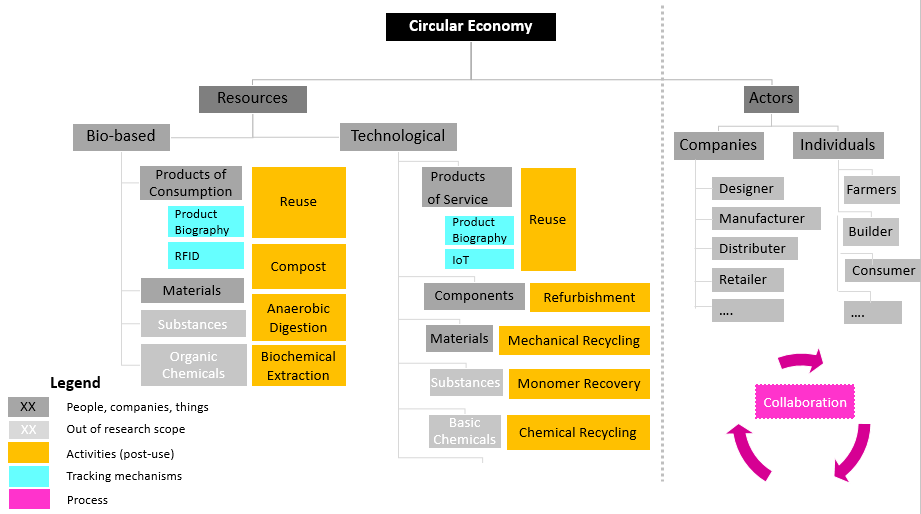
\includegraphics[width=\maxwidth{\textwidth}]{./img/image1.png}
\cprotect\caption{Example Circular Economy Taxonomy}
\label{_Ref488732938}
\end{figure}


Resources and actors are key elements for the circular economy (grey).  Actors are the different companies or individuals. Resources are divided into two main CE categories: {\bf bio-based} and {\bf technological}. Resources are further broken down into a hierarchy of parts, starting with the whole part ({\bf product}) ending with the smaller part ({\bf chemicals,} out of research scope). Even though products may consist of components, sometimes components can be considered as products elsewhere in the supply chain. When resources finish their use cycles, they must undergo different {\bf post-use activities} (yellow); there are some restrictions for the post-use activities' input materials i.e. only bio-based materials can be composted. Further, each product is tracked through a product biography using {\bf RFID} or {\bf IoT} technologies (cyan). Finally, `collaboration' is a process occurring between companies and individuals (pink). 

\subsection{Ontologies}

The Circular Economy ontology will be developed with products as the main focus unit, since product passports will account for the main data source. The passports should store information about the product provenance and the product qualities.
\begin{itemize}
\item {\bf Product provenance:} a supply chain sequence that details the companies or individuals involved in the product's creation. This will link to the company's profile which annotates the company's location, inputs, outputs, certifications (i.e. Fair Trade) and post-use activities (along with the reverse logistics mechanisms) offered by the company. Moreover, for the product's use stage, the owner will be annotated for the different use cycles.
\item {\bf Product Qualification: }the characteristics related to the availability, condition and location of a product are stored  \cite{_Ref490914619}. This section will also annotate possible post-use activities for a product which will ultimately link to the post-use activities offered by companies.
\end{itemize}

The following {\bf competency questions }incorporate the previous concepts and determine the scope of the ontology that will be developed:
\begin{itemize}
\item Which companies produce a jeans (product) composed of recycled denim (material)?
\item Which companies generate outputs (blue dyed water) that can be used as input by Mud Jeans (company) for repairing (activity) jeans (product)?
\item Which products (jeans) are in good state (condition) and are available for reuse (post-use activity) on a specific city (Utrecht)?
\end{itemize}

Fig.~\ref{_Ref490855958} shows a representation of the Circular Economy Ontology.  Actors and products will be related through the post use-activities, and the product provenance. Spatial features will be created for the actors' and products' locations, and the reverse logistics network.
\begin{figure}[h!]
\centering

\includegraphics[width=\maxwidth{\textwidth}]{./img/image2.png}
\cprotect\caption{Circular Economy Ontology}
\label{_Ref490855958}
\end{figure}


Extending the Good Relations  \cite{_Ref490914813} ontology will be considered by adding extra properties to the BusinessEntity (equivalent to actor) and ProductOrService (equivalent to product) classes. For ProductOrService, the extra properties encompass the qualities, provenance, composition and its post use activity. For BusinessEntitiy, the extra properties deal with the activities offered by the company and the reverse logistics. 

Depending on how the ontology will be implemented, the CE taxonomy (Fig.~\ref{_Ref488732938}) could be converted to a dedicated ontology that works in combination with the GoodRelations extended ontology mentioned above; thus handling two separate ontologies like recommended by GoodRelations implementation. In this way, actors and their product exchanges will be kept on a more general level following the GoodRelations specifications. Whereas specific classes and instances for the post-use activity types and their corresponding inputs (bio-based or technological materials) would be encoded separately on an ontology exclusively for the CE materials and post-use activities. The advantage of this approach is that using the GoodRelations extended ontology makes use of functionalities already present in the existing ontology. Otherwise, the other approach would be to develop a complete CE ontology without extending the GoodRelations ontology. 

Finally, in terms of spatial information, resources will be annotated using the GeoSPARQL ontology  \cite{_Ref490914834} for features and geometries. 

\section{Preliminary Design-Textile Use Case}

Data from existing fashion brands' websites on recycling collection points is gathered and converted to RDF using OntoRefine by Ontotext.  Information is enriched with annotations about the company (fashion brand) and the recycling services they offer (reverse logistics). Further, the query will be posed to verify if it yields the desired answer posed by jeans owner Anne.  

\subsection{Data}

Data for recycling points is obtained from the following sources, Fig.~\ref{_Ref490913683}.
\begin{itemize}
\item Kings of Indigo and their partner Sympany with textile recycling containers.
\item Zara's retail shops part of the Clothing Collection Program.
\item Mud Jeans and their partner DPD with pick up locations for returning used jeans.
\end{itemize}
\begin{figure}[h!]
\centering
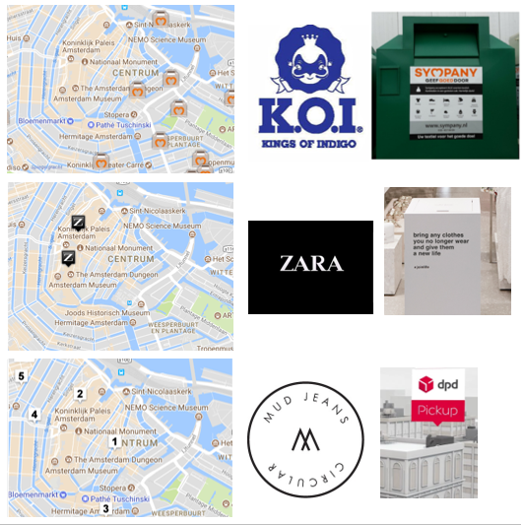
\includegraphics[width=\maxwidth{\textwidth}]{./img/image3.png}
\cprotect\caption{Example Data Sources-Recycling Collection Points}
\label{_Ref490913683}
\end{figure}


\subsection{SPARQL/GEOSPARQL query}

The question posed by jeans owner Anne, is converted to SPARQL/GEOSPARQL query language, Fig.~\ref{_Ref490912191}. 
\begin{figure}[h!]
\centering
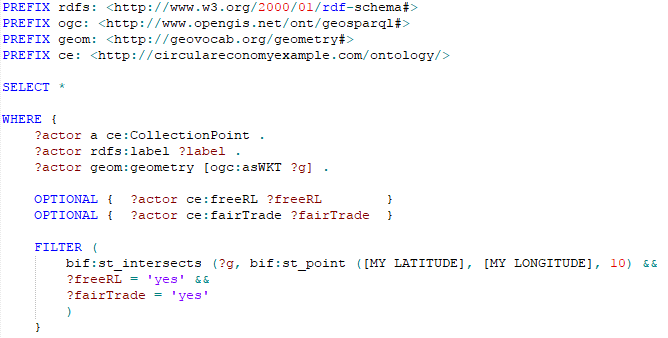
\includegraphics[width=\maxwidth{\textwidth}]{./img/image4.png}
\cprotect\caption{Example Query Fashion Use Case}
\label{_Ref490912191}
\end{figure}


\subsection{Graph Model }

A preliminary graph model that indicates how instantiated company data will take shape is shown on Fig.~\ref{_Ref488768927}. 
\begin{figure}[h!]
\centering
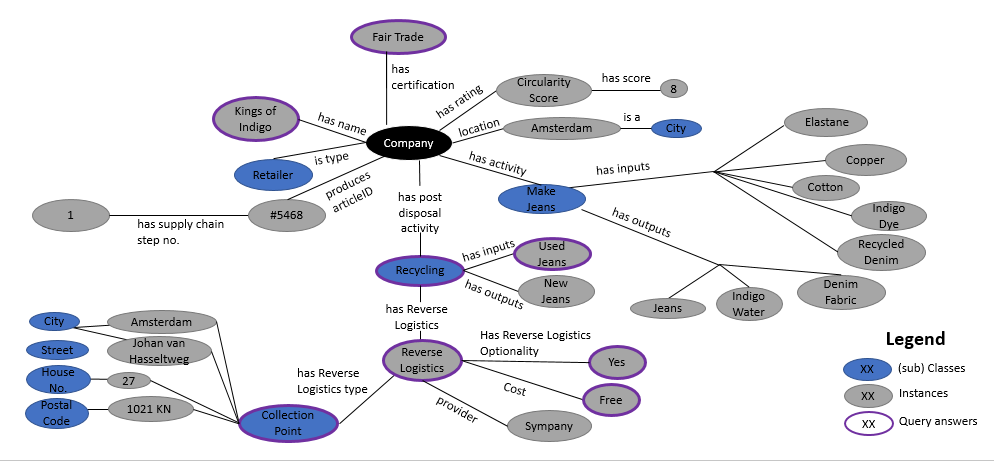
\includegraphics[width=\maxwidth{\textwidth}]{./img/image5.png}
\cprotect\caption{Fashion Graph Model}
\label{_Ref488768927}
\end{figure}


\section{Discussion}

Intended adopters of this ontology are umbrella organizations and/or governments that can lead companies and individuals in creating a Circular Economy. Under these conditions a rich, cross-industry, multi-product data environment can be created and facilitated by Linked Data. 

The heterogeneous dataset integration benefits exhibited by Linked Data make it a promising technology for meeting potential stakeholders' needs. Independent industries should maintain their own datasets as this proposition only contemplates linking and enriching them. 

Although there are relevant concerns about privacy and sensitive industry information that could be visible in this environment, this research will only handle data that is available to the public via open product passports. Control over personal information and information secrecy between economic interests are out of scope of this research and should be addressed in future works. 

The current status of the semantic technologies could present a knowledge gap for intended users such as small `circular' businesses. Further research is needed to determine what type of user interface will be most suitable for CE actors. 

\section{Future Work}

The following section details the necessary steps to continue with this research. 
\begin{enumerate}
\item Ontology: encode and implement the CE ontology.
\item Design and build: complete the textile use case with industry datasets. This involves getting material passport data, conversion to RDF format, enriching and linking the datasets. Later the creation of SPARQL/GeoSPARQL queries will be addressed.
\item Visualization of results: create a web-platform that best represents connections between people, companies, locations and things.
\item Validate the results: does this way of storing and connecting data improve collaboration when comparing it to the existing alternatives?
\item Beyond this research:
\begin{itemize}
\item Continue to find other use case applications.
\item Research on reverse logistics and route network optimization; possible integration with GIS; incorporate spatio-temporal querying. 
\item Research on industrial symbiosis and spatial clustering; possible integration with GIS suitability analyses.
\item Research on privacy and sensitive industry information.
\end{itemize}
\end{enumerate}

\begin{thebibliography}{4}

\bibitem{_Ref490914549} 3XN \& GXN Innovation. (2016). 7.Building A Circular Future. Retrieved from https://issuu.com/3xnarchitects/docs/buildingacircularfuture
\bibitem{_Ref490914691} Charpenay, V., Hund, J., Käbisch, S., \& Kamiya, T. (2017). WoT Current Practices. Retrieved May 14, 2017, from http://w3c.github.io/wot/current-practices/wot-practices.html
\bibitem{_Ref490914729} Ellen MacArthur Foundation. (2013). Towards the Circular Economy: Economic and Business Rationale for an Accelerated Transition.
\bibitem{_Ref490914619} Ellen MacArthur Foundation. (2016). 5.Intelligent Assets: Unlocking The Circular Economy Potential. Retrieved from https://www.ellenmacarthurfoundation.org/assets/downloads/publications/EllenMacArthurFoundation\_Intelligent\_Assets\_080216.pdf
\bibitem{_Ref490914294} Ghisellini, P., Cialani, C., \& Ulgiati, S. (2016). 4.A review on circular economy: the expected transition to a balanced interplay of environmental and economic systems. Journal of Cleaner Production, 114, 11--32. http://doi.org/10.1016/j.jclepro.2015.09.007
\bibitem{_Ref490914813} Hepp, M. (2008). GoodRelations: An Ontology for Describing Products and Services Offers on the Web. LNCS, 5268, 329--346. Retrieved from http://www.heppnetz.de/files/GoodRelationsEKAW2008-crc-final.pdf
\bibitem{_Ref490914646} LUCID. (2016). Linked valUe ChaIn Data --- LUCID. Retrieved May 14, 2017, from http://www.lucid-project.org/index.html
\bibitem{_Ref490914724} MBDC. (2003). Cradle to Cradle Design Guidelines.
\bibitem{_Ref490914304} Nasir, M. H. A., Genovese, A., Acquaye, A. A., Koh, S. C. L., \& Yamoah, F. (2017). 1.Comparing linear and circular supply chains: A case study from the construction industry. International Journal of Production Economics, 183, 443--457. http://doi.org/10.1016/j.ijpe.2016.06.008
\bibitem{_Ref490914641} Pawełoszek, I., Grabińska, A., \& Turek, T. (2016). Linked Data in Supply Chain Management, (April), 21--22.
\bibitem{_Ref490914834} Perry, M., \& Herring, J. (2011). GeoSPARQL - A Geographic Query Language for RDF Data | OGC. Retrieved from http://www.opengeospatial.org/standards/geosparql
\bibitem{_Ref490914539} Provenance Ltd. (2015). Blockchain: the solution for transparency in product supply chains. Retrieved May 12, 2017, from https://www.provenance.org/whitepaper
\bibitem{_Ref490914559} Remo. (2017). REMO | About. Retrieved June 28, 2017, from http://remokey.com/remo/
\bibitem{_Ref490914376} Spring, M., \& Araujo, L. (2017). 4.Product biographies in servitization and the circular economy. Industrial Marketing Management, 60, 126--137. http://doi.org/10.1016/j.indmarman.2016.07.001
\bibitem{_Ref490914370} van Buren, N., Demmers, M., van der Heijden, R., \& Witlox, F. (2016). 7.Towards a Circular Economy: The Role of Dutch Logistics Industries and Governments. Sustainability, 8(7), 647. http://doi.org/10.3390/su8070647
\bibitem{_Ref490914435} Winans, K., Kendall, A., \& Deng, H. (2017). 2.The history and current applications of the circular economy concept. Renewable and Sustainable Energy Reviews, 68, 825--833, citation p.826. http://doi.org/10.1016/j.rser.2016.09.123

\end{thebibliography}

\end{document}